\documentclass{beamer}

% Copyright 2010 Drow Ltd.
% 
% In principle, this file can be redistributed and/or modified under
% the terms of the GNU Public License, version 2.
% 
% However, this file is supposed to be a template to be modified
% for your own needs. For this reason, if you use this file as a
% template and not specifically distribute it as part of a another
% package/program, I grant the extra permission to freely copy and
% modify this file as you see fit and even to delete this copyright
% notice. 
\mode<presentation>
{
  \usetheme[titleline=true,
  alternativetitlepage=true,
  titlepagelogo=images/Java_logo]{Torino}
  \usecolortheme{nouvelle}
  \beamertemplatenavigationsymbolsempty
}

\usepackage{times}
\usepackage[utf8]{inputenc}
\usepackage[english,bulgarian]{babel}
\usepackage[T2A]{fontenc}

\usepackage{listings}
\lstset{language=Java,
  captionpos=b,
  tabsize=4,
  keywordstyle=\color{blue},
  commentstyle=\color{gray},
  stringstyle=\color{green},
  numbers=left,
  breaklines=true,
  showstringspaces=false,
  basicstyle=\ttfamily,
  emph={label},
  frame=shadowbox, 
  rulesepcolor=\color{blue},
  columns=fixed}

\title{Колекции в Java}

\author{инж. Божидар ~Бацов}

\institute{Drow Ltd.}

\date{18.01.2011}

\subject{Talks}
% This is only inserted into the PDF information catalog. Can be left
% out. 

\begin{document}

\begin{frame}
  \titlepage
\end{frame}

\begin{frame}{Съдържание}
  \tableofcontents[pausesections]
\end{frame}

\section{Въведение в колекциите}

\begin{frame}{Въведение в колекциите}
  \begin{block}{Колекции(контейнери)}
    Обект, който групира няколко елемента. Колекциите се използват за
    съхраняване, извличане, манипулиране и комуникиране на свързани
    данни. Обикновено представляват данни, които формират естествена група.
  \end{block}
  \begin{itemize}
  \item
    Стари колекции - преди Java 1.2
    \begin{itemize}
      \item Vector
      \item Hashtable
      \item array
    \end{itemize}
  \item Collections Framework
  \end{itemize}
\end{frame}

\begin{frame}{Collections Framework}
  \transdissolve
  \begin{itemize}
  \item  Унифицирана архитектура за представяне и манипулирани на
    колекции    
   \item Въведена в Java 1.2
  \item Подобна на STL в C++
  \item Включва
    \begin{itemize}
    \item интерфейси
    \item конкретни реализации
    \item алгоритми
    \end{itemize}
  \end{itemize}
\end{frame}

\begin{frame}{Предимства на Collections Framework}
  \transdissolve
  \begin{itemize}
  \item Намалява програмните усилия
  \item Увеличава скоростта на и качеството на програмите
  \item Позволява взаимодействие между различни API
  \item Намалява усилията да се учат нови API
  \item Намалява нуждата от проектиране на нови API
  \item Поощрява преизползването на код
  \end{itemize}
\end{frame}

\begin{frame}{Интерфейси}
  \transdissolve
  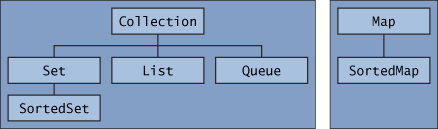
\includegraphics[height=120px,width=320px]{images/colls-coreInterfaces.png}
\end{frame}

\begin{frame}{Интерфейси}
\transdissolve
\begin{itemize}
\item всички интерфейси са генерични
\item Collection
\begin{itemize}
  \item корен на йерархията
  \item съдържа всички най-общи операции
\end{itemize}
\item Set
\begin{itemize}
  \item набор от елементи без повторения
\end{itemize}
\item List
\begin{itemize}
  \item подредена колекция от елементи
  \item може да съдържа елементи
  \item замества vector
\end{itemize}
\item Queue
\item Map 
\begin{itemize}
  \item обект, който асоциира ключове със стойности
  \item замества hashtable
\end{itemize}

\end{itemize}
\end{frame}

\begin{frame}{Имплементации}
  \transdissolve
  \begin{itemize}
  \item Стандартни имплементации
  \item Специални имплементации
  \item Паралелни имплементации
  \item Имплементации обвивки
  \item Имплементации за удобство
  \item Абстрактни имплементации
  \end{itemize}
\end{frame}


\begin{frame}{Стандартни имплементации}
  \transdissolve
  \small
  \begin{tabular}{|c|c|c|c|c|c|}
    \hline
    Int. & \multicolumn{5}{|c|}{Implementations}  \\
    \hline
    \hline
    & Hash & Resizable & Tree & Linked & Hash table + \\
    & table & array & & list & Linked List \\
    \hline
    Set & HashSet & & TreeSet & & LinkedHashSet \\
    \hline
    List & & ArrayList & & LinkedList \\
    \hline
    Queue & & & & & \\
    \hline
    Map & HashMap & & TreeMap & & LinkedHashMap \\
    \hline
  \end{tabular}

\end{frame}

\begin{frame}{Особености на стандартните имплементации}
\transdissolve
\begin{itemize}
\item реализират всички операции в съответния интерфейс
\item позволяват null елементи и ключове
\item не са thread safe
\item всички имат fail-fast итератори
\item всички са Serializable
\item всички имат публичен clone() метод
\end{itemize}
\end{frame}

\begin{frame}{Имплементации обвивки}
  \transdissolve
  \begin{itemize}
  \item Синхронизирани обвивки
  \item Непроменими обвивки
  \end{itemize}
\end{frame}

\begin{frame}{Обзор на имплементациите}
  \transdissolve
  \begin{itemize}
  \item Най-използвани
    \begin{itemize}
      \item List - ArrayList
      \item Set - HashSet
      \item Map - HashMap
      \item Queue - LinkedList   
    \end{itemize}
    \item Алтернативни имплементации трябва да се ползват само, когато
      е необходимо
    \item Класът Collections предоставя статични методи за създаване
      на обвити колекции
  \end{itemize}
\end{frame}


\begin{frame}{Алгоритми}
  \transdissolve
  \begin{itemize}
  \item Всички са събрани в класа Collections
  \item Повечето работят върху List, а не Collection
  \item Основни алгоритми
    \begin{itemize}
      \item сортиране
      \item разбъркване
      \item обръщане
      \item копиране
      \item размяна на елементи
      \item добавяне на всички елементи
      \item търсене
      \item композиция
      \item намиране на екстремуми
    \end{itemize}

  \end{itemize}
\end{frame}

\begin{frame}{Създаване на собствена колекция}
  \transdissolve
  \begin{itemize}
  \item 
  \end{itemize}
\end{frame}

\begin{frame}{Съвместимост с други API}
  \transdissolve
  \begin{itemize}
  \item Съвместимост
    \begin{itemize}
      \item upward
      \item backward
    \end{itemize}
    \item API дизайн
      \begin{itemize}
        \item Използвайте само най-общи интерфейси като тип на
          параметри на метод
        \item Използвайте най-конкретния тип за връщаната от метод стойност
      \end{itemize}
    \item Стари(Legacy) API
      \begin{itemize}
        \item Имплементирайте интерфейсите на Collections Framework за
          тях
        \item Алтернативно използвайте шаблона за дизайн Adapter
      \end{itemize}

  \end{itemize}
\end{frame}


\section*{Заключение}

\begin{frame}{Заключение}
  \transdissolve
  % Keep the summary *very short*.
  \begin{itemize}
  \item
    Java \alert{е много повече от език за програмиране}.
  \item
    JVM \alert{е целевата среда за изпълнение} на Java приложенията, а
    не физическата процесорна микроархитектура.
  \item
    За пълноценна работа с езикът и платформата Java човек трябва да
    се запознае с доста инструменти.
  \end{itemize}
  
  % The following outlook is optional.
  \vskip0pt plus.5fill
  \begin{itemize}
  \item
    Следващият път:
    \begin{itemize}
    \item
      Основния положения в езикът Java
    \item
      Повече примери, по-малко общи приказки
    \end{itemize}
  \end{itemize}
\end{frame}

\begin{frame}{Въпроси}
  \transdissolve
  \begin{center}
    \LARGEТук е момента да зададете вашите въпроси! :-)
  \end{center}
\end{frame}

\begin{frame}{Край}
  \transdissolve
  \begin{center}
    \LARGEБлагодаря Ви за вниманието!
  \end{center}
\end{frame}

\end{document}

%%% Local Variables: 
%%% mode: latex
%%% TeX-master: t
%%% End: 
